\documentclass[12pt]{report}
\usepackage[margin=2cm, left=3cm, top=2cm, bottom = 2cm]{geometry} % set margins
\usepackage{times}
\usepackage{setspace} % for line spacing
\usepackage{amsmath}
\usepackage{hyperref}
\usepackage[authordate]{biblatex-chicago}
\usepackage{sidenotes}
\usepackage{microtype}
\usepackage{siunitx}
\usepackage{titlesec}
\usepackage{pgfplots}
\usepackage{longtable}
\usepackage{tabularx}
\usepackage{multirow}
\usepackage{fancyhdr}
\usepackage{booktabs}
\usepackage{siunitx}
\usepackage{float}
\usepackage{footmisc} % for footnote size
\pgfplotsset{compat=1.16}

\titleformat{\section}
  {\normalfont\Large\bfseries} % format
  {\thesection.} % label
  {1em} % sep
  {} % before-code
\renewcommand{\thesection}{\arabic{section}}
\newcommand{\percent}{\%}
\setlength{\headheight}{15pt}
\pagestyle{fancy}
\fancyhf{} % clear all header and footer fields
\fancyhead[L]{Maxim Efimov}
\fancyfoot[L]{\today}
\fancyfoot[R]{Page \thepage}
\hypersetup{
  colorlinks,
  citecolor=black,
  filecolor=black,
  linkcolor=black,
  urlcolor=black
}

\addbibresource{Thesis.bib}

\title{Predicting real estate prices: Comparing traditional and machine learning methods}
\author{Maxim Efimov}
\date{\today}

\begin{document}
\pagenumbering{gobble} % turn off page numbering
\maketitle
\tableofcontents
\newpage
\pagenumbering{arabic} % turn on page numbering
\setstretch{1.5} % set line spacing
\fontsize{12}{18}\selectfont % set font size
\renewcommand{\footnotesize}{\fontsize{10}{12}\selectfont} % set footnote size

\newpage

\section*{Abstract}
\addcontentsline{toc}{section}{Abstract}
Employing a large empirical dataset ($n=5302$) from the Chicago area, this paper compares the performance of three econometric methods in predicting the rental price of housing units: Ordinary Least Squares (OLS) regression, Random Forest (RF) and Neural Network (NN) algorithms, represented by Adam, SGD and LBFGS solver function algorithms. The paper finds that the neighbourhood-related data points provided on modern real estate digital platforms provide a significant amount of extra goodness of fit, and that the more complicated to use, more computationally intensive algorithms provide better analysis of voluminous, complicated data with gaps, large potential for non-linear relations and hard-to interpret coefficients. More specifically, this monograph concludes that the RF algorithm performs the best ($R^2\approx 0.838$), with the NN algorithm coming second ($R^2\approx 0.82$) and OLS regression having the worst goodness-of-fit score ($R^2\approx 0.573$). The paper concludes that the RF algorithm is the best suited for the task of predicting rental prices, and that the NN algorithm is the second best, while OLS regression is the worst.


\section{Introduction}
\subsection{Background}

Real estate markets are as old as human civilisation itself, but with new technological advancements they were able to become more open, transparent, standardised and sophisticated than ever. Modern rental and house sale listing websites include a vast variety of metrics, from internal, propriety metrics like the Zillow price estimation score “Zestimate”, to third-party metrics like the “walk score” (\cite{WalkScore2024}), to landlord- and tenant-submitted information like the exact contract details and unit features. At the same time, the manifold increases in semiconductors’ computational power, as well as the gradual improvements in data analyses algorithms allow researchers to analyse the data in more sophisticated ways, untangling at times non-linear relations or non-obvious interactions between variables.

This monograph aims to combine the advantages provided by these two trends to see if modern data, provided by real estate listing websites can be used to predict the rental price of a given unit, and if so, which of the modern econometric methods is best suited for the task. The paper will focus on the Chicago area, since it is one of the largest metropolitan areas in the United States, with a large variety of housing units, and a large amount of data available for analysis.

\subsection{Literature Review}

The most common method of predicting housing prices is the hedonic pricing model, which is a regression model that takes a price of two instances of a good with different prices and characteristics, and argues that the difference in prices reveals the difference in pleasure that the two goods provide to the typical consumer. Thus, comparing two goods that differ in one characteristic and price, we can assign price to a unit of that characteristic (\cite{taylor2003}). The hedonic pricing model was first introduced by \textcite{rosen1974} and has since been used in a variety of contexts.  It is essentially a linear regression model, which means that it is limited in its ability to capture non-linear relations between the variables, and is also limited in its ability to capture interactions between the variables, while in reality we often see that a characteristic can be positive only when there is a certain amount of it and negative otherwise, it can scale pleasure exponentially or plateau after a certain amount of it possessed. Still, it provides a powerful insight into the logic behind most linear regressions, and this logic will be used when interpreting linear regression.

When it comes to machine learning methods, a few papers tried to use them to predict housing prices. \textcite{joshi2022} compared the performance of numerous machine learning algorithms on the task of predicting housing prices in the area of Bangalore, India, and found that the Random Forest (RF) algorithms performed the best, with Ordinary Least Squares (OLS) regression coming last and Neural Network (NN) algorithms not directly studied. Other studies (e.g. \textcite{zietz2008}) used OLS methods to interpret how various metrics of a given house affected its sale price. Rental prices were less studied, but \textcite{yoshida2022} came very close in its subject and scope, comparing various algorithms in their ability to predict rental prices. Of the algorithms considered in that paper, RF performed the best for every sample size considered, Adam had a middling performance, and OLS had the worst fit on all metrics and for all sample sizes (\cite[p. 19]{yoshida2022}).

\textcite{neloy2019} also had a very similar topic, comparing different algorithms, including all 3 studied here; it went into detail on each one's characteristics, and its insights were useful in understanding the mechanics behind each algorithm. This paper showed OLS regression having a very poor performance, with $R^2=0.03$\footnote{Using root mean squared error (RMSE) would be misleading, as the dependent variable for machine learning methods needs to be normalised by presenting it as a range between 0 and 1, with 1 being the maximum value of rent in the dataset}, RF with the best fit of $RMSE\approx 0.19$ and Adam solver neural network with a middling score of $RMSE\approx 0.342$. The paper also compares RF regression, run with every variable and another one, run with only numeric variables -- the difference between the two was minimal, with $RMSE_{RF\_numeric}-RMSE_{RF\_full}\approx 0.002$. Other features of the paper differed from this monograph's design: it assumed optimal hyperparameters without performing grid search, did not study the difference between fewer and more variables included for every model, and had different methods for measuring performance. The amount and types of variables used were also fairly different (\cite[p.352]{neloy2019}).

\subsection{Aim and Research Questions}
The goals of this thesis then will be to see if the neighbourhood-related data points provided on modern real estate digital platforms provide a significant amount of extra goodness of fit, and whether the more complicated to use, more computationally intensive algorithms provide better analysis of voluminous, complicated data with gaps, large potential for non-linear relations and hard-to interpret coefficients. The paper will try to answer two research questions: “Do neighbourhood characteristics reliably influence the rental price of housing units?”  with the expectation that they do, and “Which econometric prediction model uses a variety of provided data to create a prediction model with the best goodness-of-fit score?”, where the expectation is that the neural network will be best suited to make predictions based on the data, due to it being the most computationally expensive, most ``open-minded" model, able to operate with a lot fewer assumptions about the underlying data, than the other two.

This thesis can provide value by showcasing the strengths and weaknesses of each method and finding out which is the best one for analysis -- this could be useful for future researchers, who would like to use similar methods to analyse similar data. It can also provide value to the real estate market participants, who would like to know which factors are the most important when it comes to determining the rental price of a given unit and can then make better value judgments for either leasing or renting out apartment units and houses.

\section{Data}

\subsection{Data sources}

For this work, data from the Zillow rental database for the city of Chicago will be used. The full dataset on Zillow includes around 6000 listings, with the precise number varying depending on day and season of the year. Zillow was chosen due to the availability of its data and the high amount of data points available for each listing, including some that are calculated by the website itself. The dataset is not without its flaws, however -- due to the website managers' anti-AWI\footnote{Automated Web Interactors} policy, collecting the entire database proved perilous. In the end, a representative sample was selected -- it consists of random houses, taken proportionally from each rental price bracket -- see fig. \ref{fig:plot1} and \ref{fig:plot2} for comparison between the rent distribution of the dataset and the sample. Note that listings with rental prices below \$600 were excluded, since despite nominally making up a sizeable part of the overall data, they in practice consist mostly of listings with unspecified rent price, or a placeholder that will then have to be renegotiated with the landlord.

\subsection{Data acquisition}
Data was acquired from the Zillow website using AWI techniques with the help of a browser extension called ``webscraper.io" (\cite{webscraper}). The extension allows the user to select the desired data on the website, and then automatically scrape it into a .csv file. The data was then cleaned and processed using the Python 3.11 programming language.\footnote{The code used for data acquisition and cleaning is available in the appendix.} This tool, however, has its limitations: sometimes, it does not capture all listings, especially when multiple are available for rent in one apartment complex -- nor does it always copy information of every listing on the website. For other information, such as ``facts and features", the extension creates a single unpunctuated text block, which has to be further parsed with the use of Python and regular expressions. Luckily, Zillow stores the data using a standardised format, making it simple to look for specific words and expressions, always appearing in the same place and phrased the same way for all listings, but some data is still inevitably lost in the process.

\subsection{Data description}

The resulting sample consists of N listings, each with 60 variables. The list of variables is given in table \ref{tab:variable_list}. ``Commute" here means a metric, provided by Zillow itself -- the platform allows its users to select one or several places of their current work, and the platform then plots the most efficient course for the chosen method of transportation between the unit selected and those places. This metric was used as a potentially superior and more convenient alternative to distance from the centre of the city, since it takes into consideration how traffic density and ease of transportation can affect transit from equidistant points. For the sake of this paper, the Willis Tower\footnote{Colloquially known by its former name - the Sears Tower.} was picked as a commute point -- this building is both the most well-known and tallest in Chicago, and is located in the very centre of the city's office district, the Loop. Thus, it can act as a proxy for the city centre and a popular work commute location. Categorical variables, such as flooring, allowed pets and others, were separated into boolean\footnote{Here and going forward, ``boolean" means a variable that can only take one of two values - 1 or 0.} ``dummy" variables. For a quantitative description of the existing data, see table \ref{tab:summary_statistics}.

\begin{figure}[ht]
	\centering
	\begin{tabular}{l l l l l S[table-format=3.2]}
		\hline
		                 & Min & Max  & Median & Mean    & $\sigma$ \\
		\hline
		Rent             & 575 & 4189 & 2050   & 2123.65 & 715.80   \\
		Beds             & 0   & 6    & 2      & 1.57    & 1.04     \\
		Baths            & 0.0 & 4.5  & 1      & 1.23    & 0.46     \\
		Walk-score       & 0   & 100  & 92     & 87.44   & 12.00    \\
		Transit-score    & 31  & 100  & 71     & 74.90   & 14.63    \\
		Bike-score       & 29  & 99   & 86     & 81.95   & 12.24    \\
		Footageplural    & 10  & 4089 & 900    & 916.85  & 354.14   \\
		Commute\_rush    & 2.0 & 55.0 & 24.43  & 23.34   & 10.12    \\
		Commute\_nonrush & 1.0 & 49.0 & 21.55  & 20.36   & 8.73     \\
		Arrests          & 434 & 5251 & 1503   & 1507.20 & 591.62   \\
		\hline
	\end{tabular}
	\caption{Summary statistics of the sample}
	\label{tab:summary_statistics}
\end{figure}

\subsection{Data cleaning}
During the cleaning process, listings with unstated rental price or square footage were removed. Crime rates were extrapolated from neighbourhood-wide data, provided on the website ``Neighbourhood Scout" (\cite{NeighbourhoodScoutCrime}), which collects its data from U.S. law enforcement agencies. Missing values were imputed with imputation methods differing by column, giving preference to more precise methods of imputation if possible. For instance, while the missing values in the columns ``footageplural" and ``arrests" were filled with the sample and city mean, school rating data was filled with the mean of other, non-missing ratings of the schools nearby, deposits and application fees were filled with the average for the units from the same rent bracket, since many flats' deposits and fees are set to be multiples of monthly rent (\cite{PocketSense}). Area-specific variables, such as commute time, were first imputed based on the units' postcodes, then based on the average of their neighbourhoods, and only then the still missing values were filled with the dataset's global average. Boolean ``dummies" were created for missing values -- that way, if the missing values are not distributed with the same mean as the values on which basis they are imputed, these boolean indicators will indicate this hidden relationship between rent and the missing status of values, thus lending both more predictive and more interpretation power to the models.
Those values of rent and square footage, that were outside their respective interquartile ranges, were deemed outliers and removed according to the interquartile range method of finding outliers.\footnote{More specifically, the interquartile range refers to the range between the value of the 1\textsuperscript{st} and 3\textsuperscript{rd} quartiles, and it is a common practice to remove those values that are 1.5 interquartile ranges above the third quartile or below the first quartile cut-off points, respectively (\cite{garlits2023}).}

\section{Methodology}

\subsection{Model comparison}
For the sake of comparison, data will be separated into a training and testing sub-samples. Each algorithm-dataset combination will be ``trained" on the training sub-sample, comprising 70\% of the overall data - the algorithms will make predictions based on the patterns learned from this data, be it linear regression coefficients or neuron weights. After that, each algorithm will be shown the remaining 30\% of the data - the ``testing" sub-sample; rent values of those data points will be omitted, and hence algorithms will not be able to draw further conclusions from this data. Instead, previously internalised patterns will be used by the algorithms to make their own predictions. I.e. each model will make a judgement - based on the independent variables, what is the most likely dependent variable value? Goodness of fit will be evaluated using the out-of-sample $R^2$, calculated by the following formula:
\begin{equation}
	R^2_{oos} = 1 - \frac{\sum_{i=1}^{n}(y_i - \hat{y}_i)^2}{\sum_{i=1}^{n}(y_i - \bar{y})^2}
\end{equation}
where $y_i$ is the actual value of the dependent variable, $\hat{y}_i$ is the predicted value of the dependent variable, and $\bar{y}$ is the mean of the dependent variable. The out-of-sample $R^2$ is used to avoid overfitting, which is a common problem with machine learning algorithms (\cite[p. 2]{hawinkel2023}), and to ensure that the model is able to generalise to new data, not just the data it was trained on. This method also has a welcome effect of being resilient to spurious increase in in-sample $R^2$, that manifests when extra variables are added, regardless of their effect on the dependent variable, and occurs due to the phenomenon of variance-bias trade-off in OLS models (\cite{dalpiaz2021}). Scatter plots will also be used to provide a visual summary of how the predicted variables differ from the actual variables on the same row for various values of the latter. Note that the out-of-sample $R^2$ can be negative, if the model predicts the dependent variable worse, than one that always predicts its mean value -- i.e. worse than a blind guess or a model with zero goodness-of-fit.

\subsection{Ordinary Least Squares}
Ordinary Least Squares (OLS) is a method of estimating the parameters of a linear regression model. It is a special case of the Generalized Linear Model (GLM), which is a generalization of the linear regression model, allowing for non-normal distributions of the dependent variable. OLS is a method of finding the parameters of the linear regression model, that minimize the sum of squared residuals. The model is given by the following formula:
\begin{equation}
	Y = \beta_0 + \beta_1 X_1 + \beta_2 X_2 + ... + \beta_n X_n + \epsilon
\end{equation}
where $Y$ is the dependent variable, $X_i$ are the independent variables, $\beta_i$ are the coefficients, and $\epsilon$ is the error term. To find values of \(\beta_i\) that minimize the sum of squared residuals, the following formula is used:
\begin{equation}
	\hat{\beta} = (X^T X)^{-1} X^T Y
\end{equation}
where $\hat{\beta}$ is the vector of estimated coefficients, $X$ is the matrix of independent variables, and $Y$ is the vector of the dependent variable, $T$ indicates a transposed matrix.

The OLS model, however, relies on several assumptions, which, if violated, can lead to biased estimates of the coefficients. The assumptions are as follows:
\begin{enumerate}
	\item Zero Conditional Mean: the error term has a mean of 0. This assumption is necessary for the model to be unbiased, since if the error term has a mean of 0, then the expected value of the dependent variable is equal to the expected value of the independent variables, which is the definition of an unbiased estimator (\cite{Crudu2022}). This assumption will be tested by performing a one-sample t-test on residuals.
	\item Homoscedasticity: the error term has a constant variance. This assumption is necessary for the model to be efficient, since if the error term has a constant variance, then the variance of the coefficients is also constant, which is the definition of an efficient estimator (\cite{Yang2019}). In this paper, this assumption will be tested by visually observing the scatter plot of fitted values, plotted against their residuals, and then performing a Breusch-Pagan test.
	\item Exogeneity: the error term is uncorrelated with the independent variables. This assumption is necessary for the model to be consistent, since if the error term is uncorrelated with the independent variables, then the model will converge to the true value of the coefficients as the sample size increases, which is the definition of a consistent estimator (\cite[p. 95]{Baltagi2011}). In this model, exogeneity will be tested for by regressing the residuals on the original predictors ($X_n$).
	\item Normality: the error term is normally distributed. This assumption is necessary for the model to be normally distributed, since if the error term is normally distributed, then the model will also be normally distributed, which is the definition of a normally distributed estimator (\cite{schmidt2018}). This assumption will be tested by examining a histogram of residuals' distribution and performing Shapiro-Wilk test.
	\item No Multicollinearity: the independent variables are linearly independent. This assumption is necessary for the model to be identifiable, since if the independent variables are linearly independent, then the model will be able to identify the effect of each independent variable on the dependent variable, which is the definition of an identifiable estimator (\cite{shrestha2020}). In this paper, it will be tested by visually observing a correlation matrix of all independent variables against all other variables, then creating a table of VIF values for each variable.
\end{enumerate}

Moreover, since the model assumes a linear relationship \(Y=\beta_0+\beta_n X_n\), if the underlying relationship is non-linear -- e.g. quadratic: \(Y=\beta_0 + \beta_n X_n\textsuperscript{2}\), a separate variable \(Xsquared=X\textsuperscript{2}\) has to be created to capture this relationship. The same holds true for the interaction between variables -- for instance, if $\beta_n$ only has an effect on $Y$ when $\beta_m>N$, a new variable has to be created and set to $\beta_n$ for rows where $\beta_m>N$ and 0 otherwise. This is problematic because creating an OLS model requires the creator to have accurate knowledge of the relationship between indices. Since including more variables into a regression model will always lead to better results on average (\cite{Aoki2023}), these synthetic variables should not be included without at least some level of knowledge that the relationship is non-linear, making hypothesising relationships between variables a mandatory, essential part of building any regression model.

For the sake of this thesis, no quadratic or other non-linear relationship was assumed and hence no variables were created, since the author is unaware of any literature that makes a compelling theoretical argument why a given variable in this dataset is supposed to have a non-linear relationship. It is possible that such relationships and even such arguments exist and were overlooked, but the paper's focus is to compare OLS, RF and NN regressions in their realistically achievable use cases. Since OLS is very explicit and malleable, it is always theoretically possible to explicitly define any relationship that neural networks would identify through the use of synthetic variables; in practice, however, since it requires a nearly perfect amount of forethought, it was presumed methodologically sound to compare the model with no such variables, presuming no extra knowledge of the variables' relationships to see what the model can do ``on its own".

\subsection{Random Forest}
Random Forest is a machine learning algorithm, which is used for both classification and regression tasks. It is an ensemble method, which combines multiple decision trees into a single model. The entire process cannot be summarised in a single formula, but it consists of first bootstrapping the dataset into subsets -- for the ``sklearn" library in the Python programming language, each subsample contains approximately 63.2 percent of the original dataset (\cite{Steorts15}), the rest are duplicates of these. After that, the trees are constructed by randomly selecting a subset of the data, and then selecting a subset of the variables to split on at each node (\cite[p.160]{cutler2011}). To choose the right split, the model relies on the concept of information gain, which is either calculated using Shannon information gain with this formula:
\begin{equation}
	H = -\sum_{i=1}^{n} p_i \log_2 p_i
\end{equation}
where $H$ is entropy, $p_i$ is the probability of the $i$-th class (the information gain is then calculated by subtracting the entropy of the parent node from the weighted average of the entropy of the child nodes), or using Gini impurity with the use of this formula:
\begin{equation}
	G = \sum_{i=1}^{n} p_i (1 - p_i)
\end{equation}
The split with the lowest Gini impurity is then selected. The trees are then aggregated into a single model by taking their votes -- in the case of a continuous dependent variable -- their predictions, and averaging them according to the formula:
\begin{equation}
	\hat{Y} = \frac{1}{N} \sum_{i=1}^{N} Y_i
\end{equation}
where $\hat{Y}$ is the predicted value of the dependent variable, $N$ is the number of trees, and $Y_i$ is the prediction of the $i$-th tree (\cite[p. 159]{cutler2011}). The model is then used to predict the dependent variable for new observations.
Random Forest regression allows for non-linear relationships between the dependent and independent variables, since it is a non-parametric method; nor does it require independent variables to be independent of each other (\cite{Stekhoven2011}). It also is not dependent on the assumption of normality or homoscedasticity of the error term. All of these features bring it in sharp contrast with OLS models, that rely on all the aforementioned assumptions to be able to make accurate predictions. RF models are also less prone to bias due to multicollinearity or overfitting (\cite{lindner2022}), although they are not completely immune to it. Error term, correlated with the model's independent variables may also reduce the RF models' prediction quality, though the model can still be used even if the error terms are correlated, unlike the OLS model.

The trade-off that comes in return for this more versatile model and better predictive power with ``dirty" and non-linear data is severely hampered interpretability, quite lacking in comparison with the OLS model. Here, no coefficients, variances or confidence intervals are given for each variable; fewer analytical tools are available for the model overall as well. The only metric that displays information about individual independent variables and their effects on the model is the importance factor. It is computed according to the formula:
\begin{equation}
	\frac{1}{N_{trees}} \sum_{i=1}^{N_{trees}} \sum_{t=1}^{N_{nodes}} I(v_{t} = X_j) \Delta Q_{t}
\end{equation}
where $N_{trees}$ is the number of trees in the forest, $N_{nodes}$ is the number of nodes in the $i$-th tree, $I(v_{t} = X_j)$ is the indicator function that is equal to 1 if the $j$-th variable is used to split the $t$-th node, and 0 otherwise, and $\Delta Q_{t}$ is the increase in the splitting criterion, which is either the decrease in the Gini impurity, or the decrease in the entropy. The importance factor is then scaled to sum to 1. The importance factor is then used to rank the variables in order of importance, and shows what percentage of the model's overall predictions was determined based on the influence of a given variable.

Since the random forest regression can be set up in many ways, the best parameters will be estimated using a grid search. The parameters that will be tested are the number of trees in the forest (100, 200, 300 or 1000), the maximum depth of the trees (5, 8, 15 or 25), the minimum number of samples required to split an internal node (2, 5, 10, 15, 100), the minimum number of samples required to be at a leaf node (1, 2, 5, 10), and the best criterion for split selection -- Gini impurity or the Shannon entropy's information gain. The grid search will be performed using the sklearn library in the Python programming language. This search should cover the range where a vast majority of models' loss functions plateau (\cite[p. 354]{neloy2019}).

\subsection{Neural Networks}
Neural networks are another machine learning regression, used for both classification and regression tasks. Neural networks are a set of algorithms that are designed to recognise patterns. They are inspired by the human brain, and consist of layers of neurons, which are connected to each other (\cite{shi2023}). Each neuron is a mathematical function that takes in a set of inputs, multiplies them by a set of weights, and then passes the result through an activation function. Overall, the mechanism of transmission of output of neurons is independent of the solver algorithm, and takes a form of a function:
\begin{equation}
	Y_n = f(W_n1X_1 + W_n2X_2 + ... + W_nkX_k)
\end{equation}
where $Y_n$ is the output of the $n$-th neuron, $W_n$ is the weight vector of the $n$-th neuron, $X_k$ is the $k$-th input, and $f$ is the activation function. If a neural network has multiple layers of neurons, then the previous layer's output $Y$ acts as an input $X$ to the next layer's neurons. The activation function is a function that is applied to the output of the neuron, and is used to introduce non-linearity into the model. For this paper, two activation functions will be considered -- ReLU, defined by the formula $f(x) = max(0,x)$ and tanh, defined by the formula $f(x) = \frac{e^{x}-e^{-x}}{e^{x}+e^{-x}}$. Solvers are the mechanism of updating the weights of the neurons. For this paper, three solver functions will be considered -- SDG, Adam and LBFGS.

SGD, or Stochastic Gradient Descent, is an iterative method for optimising an objective function with suitable smoothness properties. It can be used to find a local minimum of a function, and is used in machine learning to update the weights of the neurons. The algorithm works by first calculating the gradient of the loss function ($Q(w)=\frac{1}{n}\sum_{i=1}^{n}Q_i(w)$), where $w$ is the parameter that minimises $Q_i(w)$ and needs to be estimated (\cite{sra2011}), and then updating the weights of the neurons by subtracting the gradient from the weighs ($w_{k+1}=w_{k}-\eta\nabla Q_i(w)$). The algorithm is called stochastic because the gradient is calculated using a single sample, rather than the entire dataset (as opposed to $w_{k+1}=\eta\nabla Q(w_k)$), which is updating the variable based on the average of all samples, since $\eta\nabla Q(w)=w-\frac{\eta}{n}\sum_{i=1}^{n}\nabla Q_i(w)$). This is done to speed up the process of finding the minimum, and to avoid local minima. It is a gradient descent algorithm because the weights are updated in the direction of the negative gradient, which is the direction of the steepest descent.

Adam is another optimisation algorithm, which is an extension of SGD. It is an adaptive learning rate optimisation algorithm, which is used to update the weights of the neurons. It is based on adaptive estimates of lower-order moments, and is computationally efficient. Furthermore, it is also well suited for problems that are large in terms of data and/or parameters. The algorithm works by first calculating the first and second moments of the gradient, and then using them to update the weights of the neurons. The first moment is the mean of the gradient, and the second moment is the uncentred variance of the gradient. The model seeks to optimise the empirical loss function with weight decay regularisation:
\begin{equation}
	L(W) = \frac{1}{n}\sum_{i=1}^{n}L_i(W)+\frac{\lambda}{2}||W||_F^2
\end{equation}
where $W$ is the set of weights, $n$ is the number of samples, $L_i(W)$ is the loss function for the $i$-th sample given by $L_i(W)=-log\frac{e^{F_{y_i}(W,x_i)}}{\sum_{j\in(-1,1)}e^{F_j}(W,x_i)}$ for data x\textunderscore i and y\textunderscore i, and $\lambda$ is the regularisation parameter (\cite{zou2021}). The algorithm then calculates the bias-correlated first and second moments of the gradient:
\begin{equation}
	m_t = \beta_1 m_{t-1} + (1-\beta_1)g_t
\end{equation}
\begin{equation}
	v_t = \beta_2 v_{t-1} + (1-\beta_2)g_t^2
\end{equation}
\begin{equation}
	\hat{m_t} = \frac{m_t}{1-\beta_1^t}
\end{equation}
\begin{equation}
	\hat{v_t} = \frac{v_t}{1-\beta_2^t}
\end{equation}
\begin{equation}
	w_{t+1} = w_t - \frac{\eta}{\sqrt{\hat{v_t}}+\epsilon}\hat{m_t}
\end{equation}
where $m_t$ and $v_t$ are the first and second moments of the gradient at time $t$, $\hat{m_t}$ and $\hat{v_t}$ indicate that they are bias-corrected, $\beta_1$ and $\beta_2$ are the forgetting factors for the first and second moments of the gradient, $g_t$ is the gradient at time $t$, $\eta$ is the learning rate, $\epsilon$ is a small number to prevent division by zero, and $w_{t+1}$ is the updated weights at time $t+1$ (\cite{kingma2017}).

LBFGS is a limited-memory quasi-Newton optimisation algorithm, which is used to update the weights of the neurons. It is a second-order optimisation algorithm, which approximates the second derivative of the loss function using the Hessian matrix of second derivatives:
\begin{equation}
	d_{k+1} = -H_{k+1}g_{k+1}
\end{equation}
where:
\begin{equation}
	H_{k+1} = I + \frac{y_k y_k^T}{y_k^Ty_k} + \frac{s_k s_k^T}{s_k^Ty_k}+(y_k^Ty_k)v_k v_k^T
\end{equation}
and:
\begin{equation}
	v_k = \frac{s_k}{s_k^Ty_k}-\frac{y_k}{y_k^Ty_k}
\end{equation}
where $d_{k+1}$ is the direction of the descent, $g$ is the gradient of the function, $H_{k+1}$ is the approximation of the Hessian matrix, $y_k$ is the difference between the gradients at the $k$-th and $k+1$-th iterations, $s_k$ is the difference between the weights at the $k$-th and $k+1$-th iterations, and $v_k$ is the gradient at the $k$-th iteration (\cite[p. 181]{pytlak2009}).
It is a popular algorithm for optimising machine learning models, since it is faster than the standard second-order optimisation algorithm, and requires less memory. The algorithm is called limited-memory because it stores only a few vectors $x$ that represent the approximation of the Hessian matrix (which they feed into through $y_k = \nabla f(x_{k+1})-\nabla f(x_k)$ and $s_k = x_{k+1}-x_k$), rather than the entire matrix, and quasi-Newton because it uses an approximation of the Hessian matrix, rather than the actual matrix.

To decide on the best neural network regressor for this dataset, as well as to settle on the beset parameters for the regressor, a grid search will be performed. The parameters that will be tested are the number of hidden layers (1, 2, 3), the number of neurons in each hidden layer (50, 100, 200, 500), the solver (Adam, SGD and LBFGS), and learning rate (0.001, 0.01, 0.1), all combinations of which will be tested against one another. The activation function (tanh, relu), the learning rate (constant, adaptive), and the strength of the L2 regularisation term (0.0001, 0.001, 0.01) will also be tested, but using a sequential (``greedy") search.\footnote{Grid search with these parameters comprised 329 folds and took $\approx10$ hours to be performed on the machine used}

Theoretically, sequential hyperparameter tuning can miss better combinations of parameters -- e.g. since it first searches for an optimal activation function while holding learning rate constant at its default value, it is possible that the non-default value would make an even better fit together with an activation function that will be rejected for its poor performance with the default value, thus creating an overall worse fitting model, compared to if the full grid search was to be performed. Realistically, however, empirical research shows that sequential hyperparameter tuning creates largely the same hyperparameter selections, and little performance is sacrificed for a very large decrease in amount of computation required (\cite{jin2022}). Other parameters will be left at their default values, except when change was necessary -- for instance, many of Adam and SGD models with larger amount of hidden layers do not converge within the default maximum of 200 maximum iterations, so that the number of iterations for all grid searches has to be increased to 100,000. Neural networks converge faster with lower number of neuron layers in terms of number of iterations (see figure \ref{fig:nnloss}), but the complexity of each iteration increases faster than the amount of iterations needed decreases, resulting in an overall net increase in computational cost per number of layers and neurons on each layer.

\begin{figure}[ht]
	\centering
	\includegraphics[width=0.7\linewidth]{images/LossNN.png}
	\caption{Grid search results for neural network regressors}
	\label{fig:nnloss}
\end{figure}

``Warm start" is another setting in Python's ``scikit-learn" package that allows one to save calculations -- this time by starting training of the next parameter combination of a grid search from the point where the previous combination converged to a solution. It was disabled because when following the previous solution, there is a risk that if one of the networks converges to a local loss minimum, that does not coincide with the global minimum, the following models in the search will start from the same point and become ``trapped" with this suboptimal solution. Instead, it now starts from a random point each time. The amount of folds was changed to 3 to allow each fold more training data, as well as to conserve the computational resources. This value was chosen somewhat arbitrary, but studies with other search methods have shown that when the sample size allows it, 1 fold per 1000 values is sufficient to reach a relative plateau in error term (\cite{marcot2021}). After one solver is found to be better-fitting than others, additional fine-tuning will be performed.

\section{Applications}
\subsection{Ordinary Least Squares}
For ordinary least squares, data first had to be processed to be suitable for the model. Examining Variance Inflation Factors (VIF) of the variables, as well as the correlation matrix of dependent variables, it was found that the variables ``pets\textunderscore deposit", ``Commute\textunderscore nonrush", ``Commute\textunderscore rush", ``school3",``walk-score", ``bike-score", ``lease\textunderscore term", ``transit-score", ``cats\textunderscore allowed", ``pets\textunderscore allowed", ``deposit\textunderscore missing", ``application\textunderscore fee\textunderscore missing", ``application\textunderscore fee", ``school2", ``garbageincluded", \\ ``pets\textunderscore allowed\textunderscore deposit", and ``arrests" are collinear to other variables in the set and had to be removed. The Constant regression term also had to be removed due to its large VIF ($\approx416$), indicating a strong collinearity with other variables. It was, however, left in the regression model, as removing the constant term makes interpreting the coefficients a lot harder and, based on the training subset of the data, worsens the performance of the model substantially. After that, values were fitted into a model.

Creating a scatter plot graph of these values (figure \ref{fig:heteroscedasticity}) hinted, that the model may be heteroscedastic, and variances increase with the increase in the fitted values. Performing a Breusch-Pagan test confirmed that suspicion ($P_{value}\approx1e-39$). Therefore, the regression was performed with HC3 heteroscedasticity-robust standard errors. One-sample t-test, performed on the model's residuals, showed a very strong result, with ($P_{value}\approx(1-(1e-12)$). The Shapiro-Wilk test, on the other hand, indicated that the error term is not normally distributed, with $P_{value}\approx3e-18$. This indicates that the model's error term, and hence its independent variable's values, are not normally distributed. To some extent, this is to be expected -- with 60 variables, some are likely to have a non-linear relationship with rent, and since the premise of this monograph is to see how well different models untangle complex data, the reduced performance of the linear model can be seen as simply a part of the answer. Exogeneity test showed a few variables that were correlated with the error term\footnote{``school1", ``pets\textunderscore rent", ``carpet", ``deposit", ``is\textunderscore studio" and ``footageplural"} -- the variables ``carpet", ``is\textunderscore studio", ``pets\textunderscore rent" and ``deposit" could be safely removed due to their weak correlation with rent and not being essential for the model in terms of interpretability; ``footageplural" and ``school1", however, were deemed important enough due to the fact that they are highly correlated with rent ($t\approx6$ and $t\approx15$, respectively) and are intuitively very important variables in predicting rent and interpreting the model -- removing such an important variable could bring a significant degree of omitted variable bias (\cite{walsch2021}).

\begin{figure}[ht]
	\centering
	\includegraphics[width=0.8\linewidth]{./images/residuals_vs_fitted.png}
	\caption{OLS residuals, plotted against fitted values}
	\label{fig:heteroscedasticity}
\end{figure}

The resulting model showed relatively high goodness-of-fit: $R^2\approx0.573$, indicating that the model explains approximately $57.3\%$ of the rent's variance. Looking at the scatter-plot (figure \ref{fig:ols-scatterplot}) of predicted and actual values, a clear trend is visible. The regression table (table \ref{table:coefficients}) shows, how more than half of all variables are significant at the $P_{value}<0.05$ and even $P_{value}<0.01$ levels; of all boolean variables, the largest, though not necessarily the most statistically significant effect on the rent is exuded by whether the property has a pool and whether the cable television subscription is included into the rent price. Unsurprisingly, the most statistically significant effects on the rent prices are those made by a larger amount of bathrooms, pool availability and a better rating of a nearby school -- standard hallmarks of an upper-end property in a good US American neighbourhood. In fact, it is likely that in the absence of neighbourhood variables meant that a large portion of the implicit neighbourhood effect was absorbed by the nearest school's rating -- if that was true, one would expect this variable's importance to decrease when the neighbourhood variables are present. Interestingly, these results ran largely against the established knowledge on the subject -- for instance, \textcite{zietz2008} saw the presence of a pool and number of bedrooms not have a significant variable on the house price at all ($P_{value}\approx 0.58$ and $P_{value}\approx .17$, respectively).

\renewcommand{\arraystretch}{0.5}
\begin{table}[H]
	\centering
	\begin{tabular}{l S[table-format=5.4] S[table-format=4.4] l S[table-format=4.4]}
		\hline\hline \\
		                                                 & \textbf{Coefficient} & \textbf{t-value} & \textbf{P-value}           & \textbf{95\% confidence interval} \\ \hline
		\textbf{Intercept}                               & 412.6929             & 10.939           & 0.000\textsuperscript{***} & 147.934                           \\
		beds                                             & 87.5387              & 5.964            & 0.000\textsuperscript{***} & 57.552                            \\
		baths                                            & 565.5848             & 21.909           & 0.000\textsuperscript{***} & 101.228                           \\
		footageplural                                    & 0.3390               & 6.352            & 0.000\textsuperscript{***} & 0.21                              \\
		footageunknown                                   & -68.6373             & -3.071           & 0.002\textsuperscript{***} & 87.636                            \\
		school1                                          & 53.8401              & 14.804           & 0.000\textsuperscript{***} & 14.261                            \\
		is\textunderscore flexible                       & -215.9508            & -2.485           & 0.013\textsuperscript{**}  & 340.818                           \\
		electricityincluded                              & -318.6059            & -0.960           & 0.337                      & 1301.484                          \\
		waterincluded                                    & 150.2037             & 2.249            & 0.025\textsuperscript{**}  & 261.899                           \\
		gasincluded                                      & 80.8643              & 1.375            & 0.169                      & 230.557                           \\
		sewerincluded                                    & -228.8391            & -2.715           & 0.007\textsuperscript{***} & 330.498                           \\
		internetincluded                                 & 180.3006             & 2.287            & 0.022\textsuperscript{**}  & 309.165                           \\
		cableincluded                                    & 507.0600             & 3.968            & 0.000\textsuperscript{***} & 501.094                           \\
		heatincluded                                     & -206.3218            & -5.531           & 0.000\textsuperscript{***} & 146.265                           \\
		large\textunderscore dogs\textunderscore allowed & -77.2653             & -1.348           & 0.178                      & 224.841                           \\
		small\textunderscore dogs\textunderscore allowed & -79.0760             & -1.919           & 0.055\textsuperscript{*}   & 161.568                           \\
		hasgarage                                        & 28.7403              & 1.037            & 0.300                      & 108.65                            \\
		hassurfaceparking                                & -53.0986             & -1.965           & 0.049\textsuperscript{**}  & 105.952                           \\
		hasstreetparking                                 & 123.5955             & 4.121            & 0.000\textsuperscript{***} & 117.603                           \\
		hardwood                                         & -9.8965              & -0.553           & 0.580                      & 70.173                            \\
		tile                                             & -60.6082             & -1.395           & 0.163                      & 170.332                           \\
		laminate                                         & 111.0318             & 0.674            & 0.500                      & 645.867                           \\
		linoleum                                         & 26.1472              & 0.146            & 0.884                      & 702.846                           \\
		gated                                            & -57.8895             & -2.143           & 0.032\textsuperscript{**}  & 105.935                           \\
		hasftness                                        & 125.4955             & 4.775            & 0.000\textsuperscript{***} & 103.046                           \\
		haspool                                          & 530.6163             & 20.667           & 0.000\textsuperscript{***} & 100.677                           \\
		hasac                                            & 84.3410              & 3.538            & 0.000\textsuperscript{***} & 93.466                            \\
		hasdishwasher                                    & 65.7979              & 3.566            & 0.000\textsuperscript{***} & 72.347                            \\
		hasfireplace                                     & 59.5961              & 0.939            & 0.348                      & 248.987                           \\
		year\textunderscore built                        & -0.0323              & -1.661           & 0.097\textsuperscript{*}   & 0.076                             \\
		hasbalcony                                       & 35.5822              & 1.369            & 0.171                      & 101.926                           \\
		heating\textunderscore electric                  & 42.2393              & 0.636            & 0.525                      & 260.427                           \\
		heating\textunderscore gas                       & 30.0678              & 0.812            & 0.417                      & 145.146                           \\
		heating\textunderscore forced\textunderscore air & -79.6423             & -2.772           & 0.006\textsuperscript{***} & 112.65                            \\
		heating\textunderscore radiant                   & 216.4028             & 2.085            & 0.037\textsuperscript{**}  & 406.95                            \\
		heating\textunderscore baseboard                 & 0.4906               & 0.006            & 0.995                      & 312.871                           \\
		laundry\textunderscore shared                    & -62.8458             & -2.048           & 0.041\textsuperscript{**}  & 120.348                           \\
		laundry\textunderscore in\textunderscore unit    & 290.1521             & 13.712           & 0.000\textsuperscript{***} & 82.977                            \\
		\multicolumn{4}{l}{\textsuperscript{***}$p<0.01$, \textsuperscript{**}$p<0.05$, \textsuperscript{*}$p<0.1$}
	\end{tabular}
	\caption{OLS Regression Results, no neighbourhood data}
	\label{table:coefficients}
\end{table}
\renewcommand{\arraystretch}{1}

Interestingly enough, despite anticipated over-fitting, the model's performance with the neighbourhood dummies was markedly better than without, with $R^2\approx0.649$ -- the neighbourhood boolean variables were able to explain an additional 6.6\% of the rent's value. The model's performance on the test set is shown in figure \ref{fig:ols-scatterplot-neighbourhood}, and the regression summary is available on table \ref{table:ols_with_neighbourhood}\footnote{Due to its size, the regression summary was moved to the appendix}. Quite a few neighbourhoods had a significant effect on the rent value -- unsurprisingly, the neighbourhoods with larger effects were more significant, signifying a particularly luxurious or a particularly poor neighbourhood. Both models' scatter-plot graphs show visible markers of heteroscedasticity (both variances become larger with larger rent).

\begin{figure}[H]
	\begin{minipage}{0.4778\textwidth}
		\centering
		\includegraphics[width=\linewidth]{./images/predicted_vs_actualOLS.png}
		\caption{OLS predicted vs actual values, \\ no neighbourhood booleans}
		\label{fig:ols-scatterplot}
	\end{minipage}
	\begin{minipage}{0.48\textwidth}
		\centering
		\includegraphics[width=\linewidth]{./images/neighbourhood_predicted_vs_actualOLS.png}
		\caption{OLS predicted vs actual values, \\ with neighbourhood booleans}
		\label{fig:ols-scatterplot-neighbourhood}
	\end{minipage}
\end{figure}

\subsection{Random Forest}
Upon performing the grid search, it was found that the optimal number of trees is 1000, maximum depth is 25, minimum samples per leaf is 1, and the minimum samples per split is 2 for both models. For every hyperparameter, these were the most computationally expensive parameters -- on one hand, this means that the model is capable of internalising more information  gained from the more complex hyperparameter combinations without causing more overfitting. On the other, it highlights that the best hyperparameters may be more computationally expensive still, and so it could benefit from further grid searching with those more expensive parameters. However, as complexity scales exponentially with the increase in maximum depth and linearly with increase in number of trees, further search is unfeasible with the amount of calculation power that the modern equipment provides.

\begin{figure}[ht]
	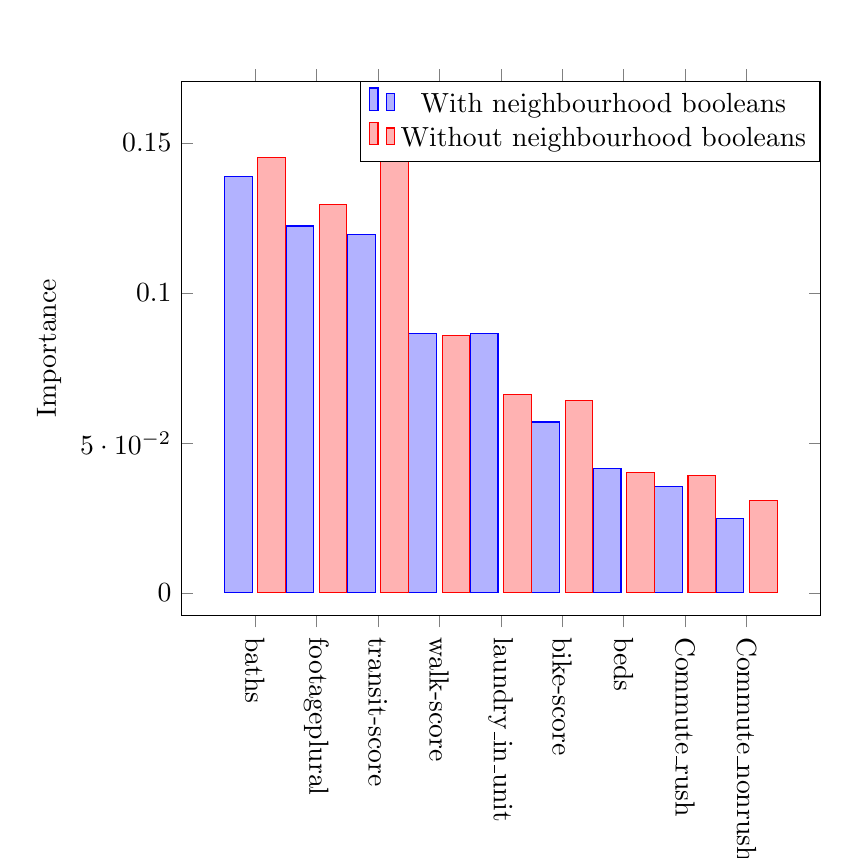
\begin{tikzpicture}
		\begin{axis}[
				width = 0.8\textwidth,
				ybar,
				enlargelimits=0.15,
				legend style={at={(1,1)},
						anchor=north east},
				ylabel={Importance},
				symbolic x coords={baths, footageplural, transit-score, walk-score, laundry\_in\_unit, bike-score, beds, Commute\_rush, Commute\_nonrush},
				xtick=data,
				ymin=0.013, ymax=0.15,
				nodes near coords align={vertical},
				x tick label style={rotate=-90, anchor=west},
			]
			\addplot coordinates {(baths,0.138816) (footageplural,0.122310) (transit-score,0.119507) (walk-score,0.086479) (laundry\_in\_unit,0.086383) (bike-score,0.056978) (beds,0.041466) (Commute\_rush,0.035334) (Commute\_nonrush,0.024675)};
			\addplot coordinates {(baths,0.145085) (footageplural,0.129590) (transit-score,0.145701) (walk-score,0.085661) (laundry\_in\_unit,0.066004) (bike-score,0.064249) (beds,0.040172) (Commute\_rush,0.039023) (Commute\_nonrush,0.030762)};
			\legend{With neighbourhood booleans, Without neighbourhood booleans}
		\end{axis}
	\end{tikzpicture}
	\caption{Feature importances for Random Forest models}
	\label{fig:rf-importances}
\end{figure}

The model's performance on the test set is shown in figure \ref{fig:rf-scatterplot-test-no-neighbourhood}. The goodness-of-fit for the model, $R^2\approx0.838$, was significantly higher, than that of the OLS model. The fact that 83.8\% of the relations between the independent variables and rent is explained by the model means that the model predicts rent with extremely high the accuracy -- the mean squared error of the predictions is 80459, meaning average rent prediction is only $\epsilon_{mean}=\sqrt{MSE}=\sqrt{80459}=283.7$ off from the actual value. The difference in goodness-of-fit between the models with and without the neighbourhood variables is relatively small, as $R^2\approx0.842$ for the model with the extra variables (see fig. \ref{fig:rf-scatterplot-test}), and the feature importance graph gives us a clue why: as we can see on figure \ref{fig:rf-importances}, not a single added variable made it to the list of 10 most important features.

In fact, the most important neighbourhood variable only ranks $26^{th}$ on the overall list. The inclusion of these booleans, however, noticeably changes the importance of other features: most features receive a lower importance score, which is to be expected since the total importance of 1 has to be divided over a larger number; the feature that gets the most deprioritised is transit score -- again, expected, since we can speculate that closeness to the centre, which has a tremendous impact on the transit quality, is closely correlated with neighbourhood values. Interestingly enough, this logic does not hold for the walk score, which becomes a little more influential -- looking at the Walk Score's explanation (\cite{WalkScore2024}) behind their Walk Score rating, it appears that it tracks how easy it is to perform daily errands without relying on public or private transport. This is still quite puzzling, as some neighbourhoods surely have a more ``walk-able" landscape, but perhaps this metric has a large variability within each neighbourhood. Having a laundry machine in the unit became much more important for the model with extra boolean variables, as this too likely does not depend on the neighbourhood of the unit and now lends more explanatory power, compared with other variables.

\begin{figure}[ht]
	\begin{minipage}[t]{0.47\textwidth}
		\centering
		\includegraphics[width=\linewidth]{./images/Predicted_vs_actual_RF_no_neighbourhood.png}
		\caption{Random Forest predicted vs actual \\ values, no neighbourhood booleans}
		\label{fig:rf-scatterplot-test-no-neighbourhood}
	\end{minipage}
	\begin{minipage}[t]{0.47\textwidth}
		\centering
		\includegraphics[width=\linewidth]{./images/Predicted_vs_actual_RF_with_neighbourhood.png}
		\caption{Random Forest predicted vs actual \\ values, with neighbourhood booleans}
		\label{fig:rf-scatterplot-test}
	\end{minipage}
\end{figure}

\subsection{Neural Networks}
For the sample without the neighbourhood booleans, grid search has shown that the best hyperparameters for the model are a constant learning rate of 0.001, 3 hidden layers with 500 neurons in each, penalty term of 0.0001, relu activation function and Adam solver function. Adam in particular allowed to perform additional fine-tuning -- the forgetting factors for the first and second moments of the gradient, $\beta_{1}$ and $\beta_{2}$ were set to 0.7 and 0.999 respectively, and the $\epsilon$ term was set to 1e-07.\footnote{Since these parameters are specific to Adam, their grid search was not explicitly discussed in methodology -- the values considered were $\beta_1=0.7, 0.8, 0.9; \beta_2=0.9, 0.99, 0.999; \epsilon=1e-08, 1e-07, 1e-06$.} The parameters of the model with neighbourhood variables was notably different in two parameters -- it found three hidden layers of 50 neurons to be more effective and opted for a larger $\epsilon$ term of 1-e6. All other metrics found through the grid search were in agreement with those that were deemed optimal by the first model's search.

These two models -- without the neighbourhood variables and with them -- have the respective out-of-sample scores of $R^2\approx0.82$ and $R^2\approx0.785$. Visual representation of their performances can be seen on figures \ref{fig:nn-scatterplot-test-no-neighbourhood} and \ref{fig:nn-scatterplot-test}. This is quite unexpected: the model that is supposed to be best at integrating large quantities of complex data is the only one that performs worse when extra data is introduced. It is possible that the grid search performed converged to a local maximum that does not represent the overall best fit, but with how extensive the parameters studied were and with ``warm start" setting disabled, it is more likely that the model became over-fitted and did not generalise as well to the test sample's data.


\begin{figure}
	\begin{minipage}[t]{0.47\textwidth}
		\centering
		\includegraphics[width=\linewidth]{./images/ScatterNN.png}
		\caption{Neural Network predicted vs actual \\ values, without neighbourhood booleans}
		\label{fig:nn-scatterplot-test-no-neighbourhood}
	\end{minipage}
	\begin{minipage}[t]{0.47\textwidth}
		\centering
		\includegraphics[width=\linewidth]{./images/neighbourhood_scatterNN.png}
		\caption{Neural Network predicted vs actual \\ values, with neighbourhood booleans}
		\label{fig:nn-scatterplot-test}
	\end{minipage}
\end{figure}

\section{Conclusion}
\subsection{Summary of Results}

As we can see in fig. \ref{fig:summary}, the Random Forest model performed the best, for both models with and without the extra boolean variables, though the difference between the RF and NN models disappears almost completely for the version without the neighbourhood booleans. Adam NN regression quality came second, and OLS -- a somewhat distant third. Knowledge of the neighbourhood of a given rental unit was found to have a very different effect on the goodness-of-fit of different regressions -- while very useful for increasing the quality of the OLS regressors, it did very little to improve the RF regression and harmed the quality of Adam regression's predictions. This cound indicate that there is somewhat of a convergence point, where worse models can benefit from more data, even if it is noisy, but the already more fine-tuned models stop benefiting as much and eventually even suffer from more noisy data included. However, it is important to note that all 3 performed reasonably well -- The worst-fit model still explained a remarkable 57.3\% of the dependent variable's fluctuations. These results mostly replicated the findings of \textcite{yoshida2022} and \textcite{neloy2019}, though this paper's results generally showed a higher goodness-of-fit across the board, possibly due to inclusion of more metrics, and the differences between the goodness of fit of different models were a lot smaller.

\begin{figure}[h]
	\centering
	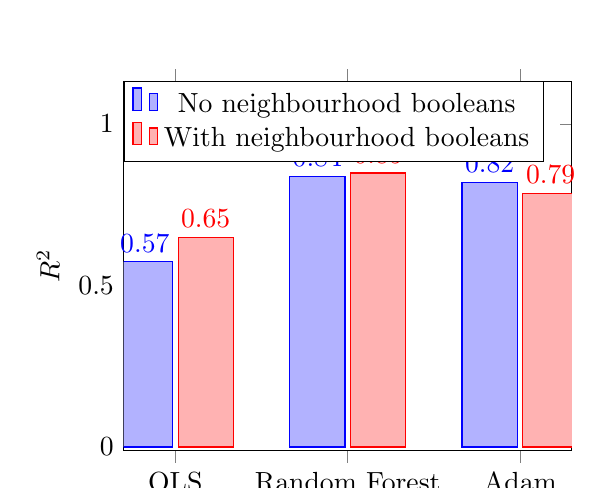
\begin{tikzpicture}
		\begin{axis}[
				width = 0.6\textwidth,
				ybar,
				bar width=20pt,
				enlargelimits=0.15,
				legend style={at={(0,1)},
						anchor=north west},
				ylabel={$R^2$},
				symbolic x coords={OLS, Random Forest, Adam},
				ymin=0.12, ymax=1,
				xtick=data,
				nodes near coords,
				nodes near coords align={vertical},
			]
			\addplot coordinates {(OLS,0.573) (Random Forest,0.838) (Adam,0.82)};
			\addplot coordinates {(OLS,0.649) (Random Forest,0.848) (Adam,0.785)};
			\legend{No neighbourhood booleans, With neighbourhood booleans}
		\end{axis}
	\end{tikzpicture}
	\caption{$R^2$ scores of the models}
	\label{fig:summary}
\end{figure}

\subsection{Limitations}
Each model came with its own list of limitations and assumptions that had to be made -- these assumptions were explained in the methodology section. Without an extremely strong computer or multiple weeks of compute time, full grid search over every possible parameter and value was completely unfeasible, and so trade-offs between potential accuracy and time had to be made. For OLS, this trade-off was irrelevant, but numerous other ones were unique to it -- as discussed above, no assumptions were made about any non-linear effects between variables, and only one instrumental variable was created. When it came to improving the model in terms of not violating its core assumptions, more judgements were made on which variables would do more harm if left in the model and which ones would damage the accuracy more if removed due to the omitted variable effect; these decisions likely had a significant effect on the model's fit.

Data availability, quantity and quality were also a significant limitation -- the dataset was limited to the city of Chicago, and even then, only to the rental units that were listed on Zillow. The dataset was also limited to the data available at the time of writing, and were there to be a strong seasonal effect on a variable, or worse yet on the relationship between the variables, the entire conclusion of the paper could be changed with further research. The models operated with the variables that were available in the dataset -- it is possible that some omitted variables would have a significant effect on the rent, and so the models would benefit from their inclusion. Perhaps the biggest challenge came from the amount of noise available in the data -- for some categorical values (e.g. flooring) some categories only appeared in less than one percent of the cases, and so effectively the sample on the basis of which models had to detect the influence these boolean variables had on rent was very small. Other variables were seldom mentioned, so the models were at risk of being influenced by a significant degree of omitted variable bias.

\subsection{Further Research}
The most obvious way to improve the models would be to increase the amount or quality of data available to them. The dataset used in this paper was limited to the city of Chicago, and even then, only to the rental units that were listed on Zillow. The dataset was also limited to the data available at the time of writing, and were there to be a strong seasonal effect on a variable, or worse yet on the relationship between the variables, the entire conclusion of the paper could be changed with further research. The models were also limited to the variables that were available in the dataset -- it is possible that some omitted variables would have a significant effect on the rent, and so the models would benefit from their inclusion. The size of the dataset could also play an important role -- \textcite{yoshida2022} showed that different sizes of the sample influence performance of the models to the great extent, and that different models may be most effective for different sample sizes. 

As mentioned in ``limitations", the models could also be improved by a more thorough grid search. This would require a more powerful computer, or a longer time to compute, but would likely result in a better fit. The models could also be improved by a more thorough analysis of the data -- for example, the relationship between the variables could be studied more closely, and the variables could be transformed to better fit the assumptions of the models. This would somewhat transform the question of the paper, shifting from studying the typical implementation of each model to their perfect implementation, but that question could also be useful to study.

Another possible way to expand the paper's scope and conclusions is to include more regression types -- perhaps instead of looking for the best solver to represent NN regressions as a whole, each could be used alongside each other and their conclusions can be compared with each other and other regression types. Other regression methods, such as LASSO, RF classifier (as opposed to regressor) and others can be included to expand conclusions and potentially draw other insights, both about the regression methods and the rental markets. XGBoost algorithm showed a lot of potential in \textcite{yoshida2022}, outperforming other algorithms with by a significant margin; if this result could be replicated, XGBoost could be tested for commercial use and potentially improve the efficiency of rental markets in a variety of ways.

\newpage
\pagenumbering{gobble}
\pagestyle{fancy}
\fancyhf{} % clear all header and footer fields
\fancyhead[L]{Maxim Efimov}
\fancyfoot[L]{\today}
\printbibliography

\appendix
\newpage

\section*{Appendix A: Data Dictionary}
\renewcommand{\arraystretch}{0.5}
\begin{longtable}{l l l}
	\hline \hline \\
	\textbf{Variable Name}                                & \textbf{Description}                                        & \textbf{Type}    \\ \hline
	\hline
	\endfirsthead
	\hline \hline \\
	\textbf{Variable name}                                & \textbf{Description}                                        & \textbf{Type}    \\ \hline
	\hline
	\endhead
	Index                                                 & Unique identifier of the listing                            & numeric          \\
	rent                                                  & Rental price of the listing                                 & numeric, \$      \\
	beds                                                  & Number of bedrooms                                          & numeric          \\
	baths                                                 & Number of bathrooms                                         & numeric          \\
	footageplural                                         & Area of the listing                                         & numeric, sq. ft. \\
	Commute\textunderscore rush                           & Average commute time to the Willis                          & numeric, min.    \\
	                                                      & tower during rush hour                                      &                  \\
	Commute\textunderscore rush                           & Average commute time to the Willis                          & numeric, min.    \\
	                                                      & tower not during rush hour                                  &                  \\
	arrests                                               & Number of arrests in the police district, 2022              & numeric          \\
	walk-score                                            & Walkability score of the listing                            & numeric          \\
	transit-score                                         & Transit score of the listing                                & numeric          \\
	bike-score                                            & Bikeability score of the listing                            & numeric          \\
	school\textunderscore 1                               & Ranking of the closest school                               & numeric          \\
	school\textunderscore 2                               & 2\textsuperscript{nd} closest school ranking                & numeric          \\
	school\textunderscore 3                               & 3\textsuperscript{rd} closest school ranking                & numeric          \\
	is\textunderscore flexible                            & Does the word ``flexible" appear                            & boolean          \\
	                                                      & in the description of the listing                           &                  \\
	lease\textunderscore term                             & Length of the contract's term                               & numeric, mon.    \\
	application\textunderscore fee                        & Fee required to apply                                       & numeric, \$      \\
	application\textunderscore fee\textunderscore missing & Is the application fee missing                              & boolean          \\
	deposit                                               & Size ofthe deposit required                                 & numeric, \$      \\
	deposit\textunderscore missing                        & Is the deposit size missing                                 & boolean          \\
	electricityincluded                                   & Are costs of electicity                                     & boolean          \\
	                                                      & included in the cost of rent                                &                  \\
	waterincluded                                         & Are costs of running water                                  & boolean          \\
	                                                      & included in the cost of rent                                &                  \\
	gasincluded                                           & Are costs of providing gas                                  & boolean          \\
	                                                      & inclued in the cost of rent                                 &                  \\
	garbageincluded                                       & Are costs of garbage removal                                & boolean          \\
	                                                      & included in the cost of rent                                &                  \\
	sewerincluded                                         & Are costs of sewer maintenance                              & boolean          \\
	                                                      & included in the cost of rent                                &                  \\
	internetincluded                                      & Are costs of internet                                       & boolean          \\
	                                                      & included in the cost of rent                                &                  \\
	cableincluded                                         & Are costs of cable television                               & boolean          \\
	                                                      & included in the cost of rent                                &                  \\
	heatingincluded                                       & Are costs of heating                                        &                  \\
	                                                      & included in the cost of rent                                &                  \\
	large\textunderscore dogs\textunderscore allowed      & Are large dogs allowed                                      & boolean          \\
	small\textunderscore dogs\textunderscore allowed      & Are small dogs allowed                                      & boolean          \\
	cats\textunderscore allowed                           & Are cats allowed                                            & boolean          \\
	is\textunderscore studio                              & Is the appartment listed as ``studio"                       & boolean          \\
	hasgarage                                             & Does the appartment come                                    & boolean          \\
	                                                      & with a garage                                               &                  \\
	hassurfaceparking                                     & Does the appartment come                                    & boolean          \\
	                                                      & with a surface parking spot                                 &                  \\
	hasstreetparking                                      & Does the appartment come                                    & boolean          \\
	                                                      & with a street parking spot                                  &                  \\
	pets\textunderscore deposit                           & Size of the pet deposit                                     & numeric, \$      \\
	pets\textunderscore allowed\textunderscore deposit    & pet\textunderscore deposit times pet\textunderscore allowed & numeric, \$      \\
	pets\textunderscore allowed                           & How many pets are allowed                                   & numeric          \\
	pets\textunderscore rent                              & What is the extra rent paid per pet                         & numeric, \$      \\
	hardwood                                              & Is the floor hardwood                                       & boolean          \\
	carpet                                                & Is the floor carpet                                         & boolean          \\
	tile                                                  & Is the floor tile                                           & boolean          \\
	laminate                                              & Is the floor laminate                                       & boolean          \\
	linoleum                                              & Is the floor linoleum                                       & boolean          \\
	gated                                                 & Is the unit located in the gated community                  & boolean          \\
	hasfitness                                            & Does the description mention a fitness centre               & boolean          \\
	haspool                                               & Does description mention a pool                             & boolean          \\
	hasac                                                 & Does the unit have an AC                                    & boolean          \\
	hasdishwasher                                         & Does the unit have a dishwashing machine                    & boolean          \\
	hasfireplace                                          & Does the unit have a furnace                                & boolean          \\
	year\textunderscore built                             & What year was it built in                                   & numeric, year    \\
	hasbalcony                                            & Does the unit have a balcony                                & boolean          \\
	heating\textunderscore electric                       & Is the heating electric                                     & boolean          \\
	heating\textunderscore gas                            & Is the heating gas                                          & boolean          \\
	heating\textunderscore forced\textunderscore air      & Is the heating done by forced air                           & boolean          \\
	heating\textunderscore radiant                        & Is the heating radiant                                      & boolean          \\
	heating\textunderscore baseboard                      & is the heating done through baseboard                       & boolean          \\
	laundry\textunderscore shared                         & Is the laundry unit shared                                  & boolean          \\
	laundry\textunderscore in\textunderscore unit         & Is the laundry done in-unit                                 & boolean          \\
	Lake View                                             & Example of a neighbourhood variable.                         & boolean          \\
	\caption{List of variables in the dataset}
	\label{tab:variable_list}
\end{longtable}

\section*{Appendix B: Data Point Distribution}


\begin{figure}[h!]
	\begin{minipage}{0.495\textwidth}
		\begin{tikzpicture}
			\begin{axis}[
					ybar,
					bar width=9pt,
					xtick=data,
					xticklabel style={rotate=270},
					xticklabels = {},
					xlabel={Rental Unit Price, USD},
					xlabel style={at={(axis description cs:0.5,-0.001)},anchor=north},
					ylabel={Listings, N},
					name=plot1,
					at={(0,0)},
					anchor=south west,
					scale only axis,
					width=0.8\textwidth,
					height=0.3\textheight
				]
				\addplot+ coordinates {(0,57) (1,287) (2,496) (3,861) (4,814) (5,790) (6,852) (7,658) (8,688) (9,576) (10,465) (11,368) (12,273) (13,240) (14,233) (15,198) (16,159) (17, 111)};
			\end{axis}
		\end{tikzpicture}
		\caption{Distribution of rental units on the \\ Zillow online repository}
		\label{fig:plot1}
	\end{minipage} % < -- this comment ensures that there is no line break between the minipages
	\begin{minipage}{0.5\textwidth}
		\begin{tikzpicture}
			\begin{axis}[
					ybar,
					bar width=9pt,
					xtick=data,
					xticklabel style={rotate=270},
					xticklabels ={},
					xlabel={Rental Unit Price, USD},
					xlabel style={at={(axis description cs:0.5,-0.001)},anchor=north},
					ylabel={Listings, N},
					at = {(0,0)},
					anchor=south west,
					scale only axis,
					width=0.8\textwidth,
					height=0.3\textheight
				]
				\addplot+ coordinates {(0,18) (1,140) (2,235) (3,463) (4,618) (5,491) (6,620) (7,588) (8,518) (9,561) (10,316) (11,156) (12,91) (13,82) (14,120) (15,114) (16, 100) (17, 71)};
			\end{axis}
		\end{tikzpicture}
		\caption{Distribution of rental units in the sample \\}
		\label{fig:plot2}
	\end{minipage}
\end{figure}

\section*{Appendix C: Regression Results -- with neighbourhood Variables}

\begin{longtable}{l S[table-format=6.4] S[table-format=3.4] l S[table-format=4.4]}
	\hline \hline \\
	                             & \textbf{Coefficient} & \textbf{t-value} & \textbf{P-value}           & \textbf{95\% confidence interval} \\ \hline
	\endfirsthead
	\hline \hline \\
	                             & \textbf{Coefficient} & \textbf{t-value} & \textbf{P-value}           & \textbf{95\% confidence interval} \\ \hline
	\endhead
	const                        & 655.9974             & 20.204           & 0.000\textsuperscript{***} & 127.319                           \\
	beds                         & 221.0305             & 22.992           & 0.000\textsuperscript{***} & 37.695                            \\
	baths                        & 504.1848             & 27.549           & 0.000\textsuperscript{***} & 71.765                            \\
	footageplural                & 0.0045               & 1.018            & 0.309                      & 0.017                             \\
	footageunknown               & -114.0932            & -4.996           & 0.000\textsuperscript{***} & 89.554                            \\
	Rosemoor                     & -710.5832            & -2.32            & 0.020\textsuperscript{**}  & 1201.03                           \\
	Roseland                     & -565.271             & -3.896           & 0.000\textsuperscript{***} & 568.93                            \\
	Avalon Park                  & -572.4482            & -2.641           & 0.008\textsuperscript{***} & 850.066                           \\
	West Pullman                 & -263.9983            & -1.366           & 0.172                      & 757.942                           \\
	Wicker Park                  & 279.462              & 1.934            & 0.053\textsuperscript{*}   & 566.732                           \\
	Douglas Park                 & -428.5483            & -2.213           & 0.027\textsuperscript{**}  & 759.293                           \\
	West Town                    & 146.9583             & 2.706            & 0.007\textsuperscript{***} & 212.934                           \\
	Old Town                     & 610.1825             & 7.136            & 0.000\textsuperscript{***} & 335.289                           \\
	Gresham                      & -579.9721            & -6.43            & 0.000\textsuperscript{***} & 353.7                             \\
	Noble Square                 & 338.6805             & 2.462            & 0.014\textsuperscript{**}  & 539.453                           \\
	Humboldt Park                & -101.4535            & -1.28            & 0.201                      & 310.899                           \\
	Bucktown                     & 127.8769             & 1.405            & 0.160                      & 356.866                           \\
	South Shore                  & -496.6453            & -8.282           & 0.000\textsuperscript{***} & 235.143                           \\
	West Loop Gate               & 372.77               & 3.546            & 0.000\textsuperscript{***} & 412.205                           \\
	Burnside                     & -660.4032            & -2.155           & 0.031\textsuperscript{**}  & 1201.958                          \\
	Ravenswood                   & -79.3973             & -1.207           & 0.227                      & 257.932                           \\
	The Loop                     & 220.8093             & 5.29             & 0.000\textsuperscript{***} & 163.679                           \\
	Logan Square                 & 99.4337              & 1.903            & 0.057\textsuperscript{*}   & 204.876                           \\
	Lincoln Park                 & -19.2649             & -0.292           & 0.770                      & 258.785                           \\
	North Center                 & -294.7727            & -2.242           & 0.025\textsuperscript{**}  & 515.502                           \\
	Lincoln Square               & 87.6699              & 0.57             & 0.569                      & 602.832                           \\
	Cragin                       & -356.0392            & -2.017           & 0.044\textsuperscript{**}  & 692.148                           \\
	Montclare                    & -743.0798            & -4.035           & 0.000\textsuperscript{***} & 722.187                           \\
	East Garfield Park           & -344.8634            & -2.748           & 0.006\textsuperscript{***} & 492.093                           \\
	Irving Park                  & -257.8675            & -2.885           & 0.004\textsuperscript{***} & 350.433                           \\
	Belmont Gardens              & -357.8251            & -1.828           & 0.068\textsuperscript{*}   & 767.608                           \\
	Uptown                       & -224.2192            & -4.826           & 0.000\textsuperscript{***} & 182.174                           \\
	South East Ravenswood        & 220.9811             & 0.502            & 0.616                      & 1727.062                          \\
	Portage Park                 & -192.3914            & -2.053           & 0.040\textsuperscript{**}  & 367.515                           \\
	River North                  & 370.4122             & 9.206            & 0.000\textsuperscript{***} & 157.776                           \\
	Streeterville                & 264.2067             & 4.452            & 0.000\textsuperscript{***} & 232.711                           \\
	Kenwood                      & -247.403             & -2.042           & 0.041\textsuperscript{**}  & 475.076                           \\
	Bronzeville                  & -235.4291            & -3.23            & 0.001\textsuperscript{***} & 285.804                           \\
	South Austin                 & -483.302             & -6.495           & 0.000\textsuperscript{***} & 291.794                           \\
	North Austin                 & -568.4002            & -2.632           & 0.009\textsuperscript{***} & 846.975                           \\
	Edgewater                    & -140.095             & -2.031           & 0.042\textsuperscript{**}  & 270.518                           \\
	Washington Park              & -588.2814            & -4.669           & 0.000\textsuperscript{***} & 494.027                           \\
	Chicago Lawn                 & -558.1016            & -2.237           & 0.025\textsuperscript{**}  & 978.295                           \\
	Woodlawn                     & -474.5569            & -5.294           & 0.000\textsuperscript{***} & 351.49                            \\
	Gage Park                    & -696.4691            & -2.286           & 0.022\textsuperscript{**}  & 1194.48                           \\
	Galewood                     & -209.5972            & -0.834           & 0.404                      & 985.487                           \\
	Grand Crossing               & -361.2181            & -2.748           & 0.006\textsuperscript{***} & 515.486                           \\
	Park Manor                   & -513.9012            & -4.276           & 0.000\textsuperscript{***} & 471.304                           \\
	Marquette Park               & -605.901             & -3.137           & 0.002\textsuperscript{***} & 757.302                           \\
	West Ridge                   & -472.4621            & -5.282           & 0.000\textsuperscript{***} & 350.776                           \\
	Greektown                    & -187.1175            & -1.052           & 0.293                      & 697.201                           \\
	Printers Row                 & -41.473              & -0.352           & 0.725                      & 462.47                            \\
	Winneconna Parkway           & -854.4718            & -1.984           & 0.047\textsuperscript{**}  & 1688.724                          \\
	South Chicago                & -537.1483            & -5.054           & 0.000\textsuperscript{***} & 416.723                           \\
	East Chatham                 & -83.8726             & -0.412           & 0.680                      & 798.35                            \\
	Chatham                      & -479.2946            & -3.3             & 0.001\textsuperscript{***} & 569.515                           \\
	Cabrini Green                & 75.4026              & 0.302            & 0.763                      & 980.308                           \\
	Brainerd                     & -554.2614            & -2.218           & 0.027\textsuperscript{**}  & 979.692                           \\
	Wrigleyville                 & 192.5017             & 0.774            & 0.439                      & 975.239                           \\
	New Eastside                 & 306.0595             & 4.014            & 0.000\textsuperscript{***} & 298.967                           \\
	Near West Side               & 127.8613             & 1.982            & 0.048\textsuperscript{**}  & 253.004                           \\
	Illinois Medical District    & 256.1884             & 1.315            & 0.188                      & 763.7                             \\
	Fulton River District        & 267.1137             & 2.024            & 0.043\textsuperscript{**}  & 517.597                           \\
	Old Town Triangle            & -361.0369            & -1.924           & 0.054\textsuperscript{*}   & 735.766                           \\
	Albany Park                  & -158.1145            & -1.154           & 0.249                      & 537.373                           \\
	Lake Meadows                 & -650.355             & -5.918           & 0.000\textsuperscript{***} & 430.954                           \\
	Mount Greenwood              & -939.5937            & -3.055           & 0.002\textsuperscript{***} & 1206.004                          \\
	River West                   & 433.1783             & 4.366            & 0.000\textsuperscript{***} & 389.061                           \\
	Goose Island                 & -174.9647            & -1.069           & 0.285                      & 641.602                           \\
	South Commons                & -407.4178            & -1.336           & 0.182                      & 1195.782                          \\
	University Village L. Italy  & -76.5543             & -0.773           & 0.440                      & 388.527                           \\
	O'Hare                       & -528.1809            & -2.691           & 0.007\textsuperscript{***} & 769.612                           \\
	North Kenwood                & -61.8776             & -0.29            & 0.772                      & 837.662                           \\
	Groveland Park               & -832.7446            & -1.924           & 0.054\textsuperscript{*}   & 1697.539                          \\
	Eden Green                   & -1140.4119           & -3.724           & 0.000\textsuperscript{***} & 1200.732                          \\
	Brighton Park                & -659.0075            & -3.738           & 0.000\textsuperscript{***} & 691.241                           \\
	Beverly                      & 599.3299             & 4.786            & 0.000\textsuperscript{***} & 491.032                           \\
	Morgan Park                  & -306.6945            & -1.979           & 0.048\textsuperscript{**}  & 607.825                           \\
	East Beverly                 & -138.7272            & -0.604           & 0.546                      & 900.625                           \\
	Pilsen                       & -176.6382            & -1.524           & 0.127                      & 454.368                           \\
	Andersonville                & 1.37E-12             & 3.74E+00         & 0.000\textsuperscript{***} & 1.44E-12                          \\
	Washington Heights           & 716.5847             & 2.356            & 0.019\textsuperscript{**}  & 1192.879                          \\
	Heart of Chicago             & -41.4534             & -0.303           & 0.762                      & 536.482                           \\
	Hermosa                      & 154.7638             & 0.947            & 0.343                      & 640.535                           \\
	Back of the Yards            & -853.8838            & -3.938           & 0.000\textsuperscript{***} & 850.239                           \\
	Little Village               & -409.2261            & -3.277           & 0.001\textsuperscript{***} & 489.679                           \\
	Schorsch Forest View         & -517.2382            & -1.189           & 0.235                      & 1706.434                          \\
	Avondale                     & -100.6952            & -1.081           & 0.280                      & 365.17                            \\
	Bridgeport                   & -599.2483            & -5.667           & 0.000\textsuperscript{***} & 414.63                            \\
	Oakland                      & -4.98E-13            & -1.35E+00        & 0.179                      & 1.45E-12                          \\
	West Humboldt Park           & -495.6704            & -2.165           & 0.030\textsuperscript{**}  & 897.651                           \\
	Scottsdale                   & 915.8017             & 2.131            & 0.033\textsuperscript{**}  & 1685.046                          \\
	West Englewood               & -66.1405             & -0.281           & 0.779                      & 922.539                           \\
	Englewood                    & -612.2485            & -6.675           & 0.000\textsuperscript{***} & 359.687                           \\
	West Chesterfield            & -118.5067            & -0.476           & 0.634                      & 977.259                           \\
	Ashburn                      & 264.9216             & 0.616            & 0.538                      & 1685.287                          \\
	Wrightwood                   & 491.8998             & 2.28             & 0.023\textsuperscript{**}  & 845.998                           \\
	West Chatham                 & -213.8942            & -0.633           & 0.527                      & 1325.308                          \\
	Jeffery Manor                & -733.4115            & -2.398           & 0.017\textsuperscript{***} & 1199.259                          \\
	Ukrainian Village            & 89.3118              & 1.06             & 0.289                      & 330.412                           \\
	Canaryville                  & -574.5012            & -1.324           & 0.185                      & 1701.132                          \\
	West Garfield Park           & -510.3422            & -1.184           & 0.236                      & 1689.931                          \\
	Lake Calumet                 & 122.06               & 0.401            & 0.689                      & 1194.656                          \\
	West Woodlawn                & -12.1305             & -0.072           & 0.943                      & 661.079                           \\
	Ravenswood Manor             & -270.9307            & -0.865           & 0.387                      & 1227.887                          \\
	O'Hare International Airport & 64.0131              & 0.135            & 0.892                      & 1855.135                          \\
	Fernwood                     & -1163.1092           & -2.698           & 0.007\textsuperscript{***} & 1690.212                          \\
	Tri-Taylor                   & -209.5938            & -1.6             & 0.110                      & 513.529                           \\
	South Deering                & -598.5159            & -1.966           & 0.049\textsuperscript{***} & 1193.866                          \\
	East Side                    & -500.7076            & -2.313           & 0.021\textsuperscript{***} & 848.931                           \\
	Magnolia Glen                & -200.3719            & -0.466           & 0.641                      & 1685.104                          \\
	Lawndale                     & -379.2828            & -2.474           & 0.013\textsuperscript{**}  & 601.27                            \\
	Hegewisch                    & -394.9539            & -1.293           & 0.196                      & 1197.618                          \\
	Marynook                     & -404.0959            & -1.322           & 0.186                      & 1198.948                          \\
	Dearborn Park                & -394.9707            & -1.828           & 0.068\textsuperscript{*}   & 847.393                           \\
	East Pilsen                  & 253.3961             & 0.926            & 0.355                      & 1073.146                          \\
	Roscoe Village               & -127.0969            & -0.657           & 0.512                      & 759.148                           \\
	Bowmanville                  & -321.5011            & -0.747           & 0.455                      & 1688.715                          \\
	McKinley Park                & -350.281             & -1.983           & 0.047                      & 692.806                           \\
	Heart of Italy               & -486.6681            & -1.597           & 0.110                      & 1194.928                          \\
	Budlong Woods                & -250.5953            & -0.819           & 0.413                      & 1199.224                          \\
	Belmont Central              & -19.6723             & -0.102           & 0.919                      & 758.569                           \\
	Chinatown                    & -664.4082            & -2.178           & 0.029\textsuperscript{**}  & 1196.199                          \\
	The Gap                      & -1.51E-13            & -5.04E-01        & 0.614                      & 1.17E-12                          \\
	Hollywood Park               & -240.5798            & -0.56            & 0.576                      & 1685.647                          \\
	Fifth City                   & -771.7465            & -2.532           & 0.011\textsuperscript{**}  & 1195.033                          \\
	West Lawn                    & 2.37E-13             & 9.07E-01         & 0.365                      & 1.02E-12                          \\
	Parkview                     & -943.3884            & -2.193           & 0.028\textsuperscript{**}  & 1686.527                          \\
	LeClaire Courts              & 45.6694              & 0.15             & 0.881                      & 1195.578                          \\
	Jefferson Park               & -490.3383            & -3.181           & 0.001\textsuperscript{***} & 604.441                           \\
	Ravenswood Gardens           & 99.3334              & 0.229            & 0.819                      & 1704.351                          \\
	Archer Heights               & 4.32E-14             & 1.70E-01         & 0.865                      & 9.98E-13                          \\
	North Park                   & 141.9964             & 0.33             & 0.741                      & 1686.424                          \\
	Garfield Ridge               & -518.7781            & -2.074           & 0.038\textsuperscript{**}  & 980.72                            \\
	Union Ridge                  & -646.0239            & -1.499           & 0.134                      & 1690.014                          \\
	West Elsdon                  & 859.3342             & 2.822            & 0.005\textsuperscript{***} & 1194.232                          \\
	Brynford Park                & 3.41E-13             & 1.44E+00         & 0.151                      & 9.33E-13                          \\
	Norwood Park West            & -413.6709            & -0.959           & 0.337                      & 1691.021                          \\
	Arcadia Terrace              & -200.2655            & -0.462           & 0.644                      & 1699.641                          \\
	Edgebrook                    & -259.6306            & -0.844           & 0.399                      & 1206.749                          \\
	Norwood Park East            & -357.1376            & -1.174           & 0.240                      & 1192.645                          \\
	Clearing                     & -105.2124            & -0.422           & 0.673                      & 978.291                           \\
	Sauganash                    & 244.95               & 0.569            & 0.569                      & 1688.122                          \\
	Edgewater Glen               & -44.263              & -0.141           & 0.888                      & 1227.174                          \\
	Chrysler Village             & 2.90E-13             & 1.31E+00         & 0.190                      & 8.65E-13                          \\
	Edison Park                  & -632.7096            & -2.898           & 0.004\textsuperscript{***} & 856.007                           \\
	Belmont Heights              & 1.06E-13             & 5.01E-01         & 0.616                      & 8.29E-13                          \\
	Belmont Terrace              & 2.80E-13             & 1.84E+00         & 0.067                      & 5.98E-13                          \\
	Stony Island Park            & -6.24E-13            & -2.84E+00        & 0.005                      & 8.57E-13                          \\
	Calumet Heights              & -296.5026            & -0.973           & 0.331                      & 1194.93                           \\
	Longwood Manor               & -448.1097            & -1.04            & 0.298                      & 1689.302                          \\
	school1                      & 53.8862              & 12.811           & 0.000\textsuperscript{***} & 16.494                            \\
	is\_flexible                 & -149.7512            & -2.24            & 0.025\textsuperscript{**}  & 262.097                           \\
	electricityincluded          & -74.5005             & -0.395           & 0.693                      & 739.407                           \\
	waterincluded                & 41.8356              & 0.686            & 0.492                      & 238.973                           \\
	gasincluded                  & -50.9072             & -0.684           & 0.494                      & 291.884                           \\
	sewerincluded                & -92.7012             & -1.215           & 0.225                      & 299.283                           \\
	internetincluded             & 81.1362              & 1.15             & 0.250                      & 276.592                           \\
	cableincluded                & 476.2642             & 4.012            & 0.000\textsuperscript{***} & 465.45                            \\
	heatincluded                 & -72.4357             & -1.473           & 0.141                      & 192.888                           \\
	large\_dogs\_allowed         & -114.535             & -0.848           & 0.397                      & 529.658                           \\
	small\_dogs\_allowed         & -59.6175             & -1.461           & 0.144                      & 160.017                           \\
	hasgarage                    & -55.789              & -2.099           & 0.036                      & 104.206                           \\
	hassurfaceparking            & -4.983               & -0.18            & 0.857                      & 108.78                            \\
	hasstreetparking             & 151.1151             & 4.944            & 0.000\textsuperscript{***} & 119.848                           \\
	hardwood                     & 35.8248              & 2.079            & 0.038\textsuperscript{**}  & 67.579                            \\
	tile                         & 88.2833              & 2.07             & 0.039\textsuperscript{**}  & 167.27                            \\
	laminate                     & 300.3473             & 3.4              & 0.001\textsuperscript{***} & 346.396                           \\
	linoleum                     & 29.16                & 0.163            & 0.870                      & 699.58                            \\
	gated                        & -31.9433             & -1.186           & 0.236                      & 105.611                           \\
	hasftness                    & 65.3727              & 2.624            & 0.009\textsuperscript{***} & 97.693                            \\
	haspool                      & 476.9952             & 20.907           & 0.000\textsuperscript{***} & 89.466                            \\
	hasac                        & 86.4721              & 3.85             & 0.000\textsuperscript{***} & 88.08                             \\
	hasdishwasher                & 31.3732              & 1.722            & 0.085\textsuperscript{*}   & 71.448                            \\
	hasfireplace                 & 103.9704             & 2.112            & 0.035\textsuperscript{**}  & 193.021                           \\
	year\_built                  & -0.0123              & -0.709           & 0.478                      & 0.068                             \\
	hasbalcony                   & 27.8488              & 1.123            & 0.262                      & 97.263                            \\
	heating\_electric            & 42.881               & 0.78             & 0.435                      & 215.476                           \\
	heating\_gas                 & 31.3631              & 0.937            & 0.349                      & 131.276                           \\
	heating\_forced\_air         & -44.0336             & -1.473           & 0.141                      & 117.223                           \\
	heating\_radiant             & 98.9614              & 0.64             & 0.522                      & 605.991                           \\
	heating\_baseboard           & 17.9248              & 0.272            & 0.786                      & 258.4                             \\
	laundry\_shared              & -102.5262            & -3.244           & 0.001\textsuperscript{***} & 123.925                           \\
	laundry\_in\_unit            & 253.7189             & 12.953           & 0.000\textsuperscript{***} & 76.809                            \\
	\multicolumn{4}{l}{\textsuperscript{***}$p<0.01$, \textsuperscript{**}$p<0.05$, \textsuperscript{*}$p<0.1$}                             \\
	\caption{OLS Regression Results, no neighbourhood data}
	\label{table:ols_with_neighbourhood}
\end{longtable}

\end{document}
